Patient-generated longitudinal biomedical data is being produced at an increasing rate. These data are more dynamic and can better represent current patient health conditions. Bionus \phware\ is an effort to perform multidimensional analyses of such data to improve health outcomes by making patient-generated longitudinal data first-class data for creating a personalized, unified, coherent, and semantically-informed personalized data analyzer. Such an analyzer can be used in real-time by patients, and patient healthcare providers to improve the accuracy of diagnoses, treatments, and improve the overall quality of patient health at a lower cost.

\phware\ provides a wearable ring or finger-clip to measure vital signs. These devices are non-invasive, non-intrusive, and  communicate with a smartphone via Bluetooth using a simple application. The smartphone application uploads the sensor data to the AI cloud services for storage and analysis. The AI cloud services performs an ensemble of algorithms and machine learning to increase the accuracy of values it assigns to vital signs \cite{Altschul2004PredictiveMI,10.2307/2984877,10.5555/1643031.1643047}. Early accuracy validation for a consumer product version of \phware\ is within tolerance for medical use for oxygen saturation, respiration rate, temperature, heart rate/variability, and sys/diastolic blood pressures.

The \phware\ consumer product, assuming an eventual approval for medical application, is being explored as a means for remote patient monitoring systems as part of the short term and long term response to the COVID-19 global pandemic with the goal to improve the quality of healthcare services delivery at the point of care for COVID-19 outpatients. New development includes a highly usable web-based dashboard for providers to review vital sign trends and an alert for outpatients whose vital signs trends indicate elevated risk. 

\subsection{Conceptual Work Problem}
\begin{figure*}
  \begin{center}
    \begin{tabular}{c}
      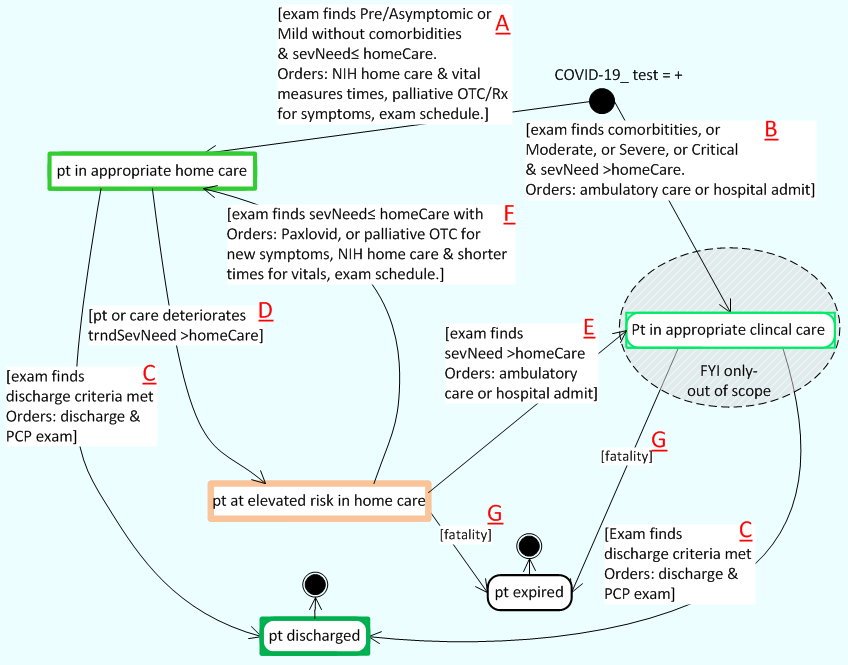
\includegraphics[scale=0.35]{cwp.png}
    \end{tabular}
  \end{center}
\caption{The CWP for remote COVID-19 patient care.}
\label{fig:cwp}
\end{figure*}

The fundamental purpose of the \phware\ system is to establish and maintain providers' timely awareness of outpatients' conditions and risk at home care; thereby, enhancing patient safety with better decisions that deliver precise care. The purpose is, however, abstract, intangible, and needs a more rigorous definition than common knowledge or intuition provides. 

The needed rigor is accomplished with a CWP, and the CWP becomes the verification requirement for the workflow model that is used as a certification that it accomplishes its intended purpose of timely awareness and patient safety while in remote monitoring. This CWP is shown in \figref{fig:cwp}. It defines the risk awareness for patient safety at home, and it defines allowable actions based on the current risk awareness. In this way, the CWP is the actionable risk awareness that must be implemented by any remote patient monitoring system such as \phware. 

A CWP is a declarative specification of a complex object of work that is shared by activities in a distributed cognitive system. It makes clear the allowed transformations by the distributed activities to move the object from some initial state to a goal state. The specification provides a connection between human cognition and the design of a system such as \phware.

There are two parts to the CWP: the data defining the state of the object on the top left corner of \figref{fig:cwp}, which is risk awareness in this application, and a state transition diagram, on the right of \figref{fig:cwp}, showing the allowed transitions between the object's states from some initial state to an eventual goal state, which in this application is a group of actions that must be taken based on risk awareness.

The object state adapts the Medicare 4-point severity-of-illness ratings to represent risk as the severity level of outpatient condition and their needed level of care \cite{severity,Hornbrook2005OverviewOD}. The ratings represent a composite of the interim guidance for COVID-19 home care \cite{cdc}. The adaptation here intends to model actionable risk awareness of a patient in home care in a computationally independent model. 

The object state consists of the physician orders (\texttt{orders}), the actual severity of the patient on the 4-point scale (\texttt{sevLvl}), the level of care the patient is able to maintain, either by caring for themselves or being cared for by a caregiver, while at home (\texttt{careCapLvl}), and the trending severity conjectured from the longitudinal data remotely being monitored and analyzed between exams as provided by the AI cloud services (\texttt{trndSevLvl}).

The state transition diagram on the right of \figref{fig:cwp} shows the relevant care states with the associated risks patients can occupy and the transition conditions among them. In the initial state (top) the patient has tested positive. The arc labeled \textbf{A} occurs when an exam shows symptoms of low severity and a provider orders home care with \phware. 

Outpatients remain in appropriate home care until either an exam finds discharge criteria met and ordered (\textbf{C}), or the trending severity level is greater than their care capability level (\textbf{D}). In such cases, patients are at an \emph{elevated risk} in home care. They must not remain at an elevated risk in home care because there is a possible direct path to fatality (\textbf{G}). So a near future exam must either order admission (\textbf{E}), find their risk lower than what the analytics claimed, or make their risk lower with additional prescribed interventions (\textbf{F}). Patients who are admitted to hospital may eventually be discharged back to home care (\textbf{H}) or discharged directly (\textbf{C}). 

The declarative knowledge of the CWP specifies \emph{what} a workflow solving the CWP must accomplish without depending on \emph{how} it does it. As such, the CWP motivates the design, and then when the design is ready, the CWP is the property for formal verification that must be satisfied to prove the workflow takes requisite actions in regard to risk awareness.

\subsection{Workflow Model}
\begin{figure*}
  \begin{center}
    \begin{tabular}{c}
      \includegraphics[scale=0.55]{bpmn.png}
    \end{tabular}
  \end{center}
\caption{The workflow models for the \phware\ system.}
\label{fig:bpmn}
\end{figure*}

The \phware\ system is modeled as a collection of workflows in the \emph{Business Process Model Notation} (BPMN) \cite{BPMNSpecification}. These include workflows for the clinicians, AI cloud services, and patient-caregivers. Workflow modeling satisfies the need for effective functional integration of people and computing. A workflow is also able to preserve the medical decision authority of providers and enable the formal verification of the correctness of the end-to-end system design for outpatient safety which is the topic of this paper.

The workflow model for the \phware\ system is in \figref{fig:bpmn}. It is designed with the MATH tool-suite, \cite{workflowmodel}, to model the functionality of interacting behaviors of the clinicians, AI cloud services, and patient-caregivers. Applying and adapting BPMN to medical care in health informatics has become the focus of the recent BPM+ project within the Object Management Group \cite{bpm}. 

The functional integration in the workflow model is adapted from concurrent design engineering in aerospace where there are specific tracks for each of the multiple design disciplines that coordinate the work on a common physical design artifact \cite{10.1007/978-1-4471-1538-0_9}. The colored lanes of the workflow are the design tracks, and the CWP is the common work artifact that must be accomplished. Each affects, and is affected, by the CWP. This feature is pivotal for integrating cognitive work that is distributed over people and computers. It allows people and computers to share work on the CWP despite vast differences in the performance properties of the way they do it. 

\figref{fig:bpmn} shows the workflow of clinicians, AI cloud services, and patient-caregivers to establish and maintain risk awareness. It starts in the green clinicians lane in the upper left of the workflow with a patient with a positive test. Such a positive test initiates an exam (task 01). The red letters in the workflow correlate to transitions in the CWP in \figref{fig:cwp}. 

Hospital admission (task 03) corresponds to edges \textbf{B} and \textbf{E} in the CWP. A severity level less that two satisfies edges \textbf{A} and \textbf{F} with the workflow leading to the clinician orders for home care via \phware\ and tele-health exams augmented with real-time vitals (task 02). Discharge criteria include a second test with a negative result following the recovery period in clinic policy and cannot be met after the first exam.

The major part of the workflow begins in the bottom, salmon color, lane for the patient-caregiver. Task 04 obtains the \phware\ sensor and associated smartphone application. It then repeats recording vitals at provider-ordered time intervals (task 05) until an exam resulting in the patient being discharged or the patient expires in home health care. The raw vitals data are transmitted by the smartphone application to the AI cloud services. 

The middle metallic grey lane represents the AI cloud services where a personal data analyzer operates on the data (task 06).  The analyzer immediately sends a packet to the clinician dashboard with vital signs and trends. An alert is added if predicted trends exceed home care capability or allowed severity in home care.

The specialized dashboard for clinicians maintains risk awareness for each outpatient (right side of the top green lane). Alerts (task 07a) skip any routine delay for the clinicians' attention. The workflow is designed to preserve the clinicians' ultimate decision authority. The AI can reason that risk is elevated if it determines trending severity is greater than the home care capability, and the provider can question the reasoning, and then confirm the alert or revise it. 

If an alert is confirmed, an urgent exam is ordered (task 08a). An urgent exam may result in hospital admission (\textbf{E}). When multiple patients have alerts, the provider must prioritize outpatients based on professional knowledge and patient familiarity. The provider may also decide the trend can be controlled by adjusting orders such as more frequent vitals reporting or changing medications (\textbf{F}). If an alert is dismissed by the provider, a routine exam still may be due to be scheduled (task 08b), or it may already be scheduled to start soon. 

For non-alerts, the provider reviews vitals when time permits (task 07b) and may order a routine exam to be scheduled. Alternatively, if clinical judgment deems it appropriate, the clinicians may order an urgent exam. The decision gate \texttt{Xor11} (far right of \figref{fig:bpmn}) is where exam times are managed. If an exam is already scheduled to begin soon, then the flow returns to task 01 where the next exam is administered when the patient arrives. The result of the exam is either to discharge, admit, or resume home care with remote monitoring and newly prescribed interventions as needed.

It is not possible to manually reason about the correctness of the workflow models in taking actions on risk awareness given the concurrency in the workflow and the several asynchronous interactions with the risk awareness both to update the risk and make decisions on the risk. The adaptation of model checking to formally reason about the correctness of the system in an automated way is an important and novel contribution to verifying the functionality of joint human-computer teams. 

\begin{comment}
The rest of this paper describes the verification of the workflow against the CWP as a verification requirement. The verification is accomplished with the SPIN model checker. 

The CWP in \figref{fig:cwp} is translated into equivalent Linear Temporal Logic (LTL), and the workflow in \figref{fig:bpmn} is translated into its equivalent Promela model, where Promela is the input language for SPIN. The SPIN model checker then verifies that the workflow in its current form does indeed implement the CWP.
\end{comment}